% This file was created by tikzplotlib v0.9.8.
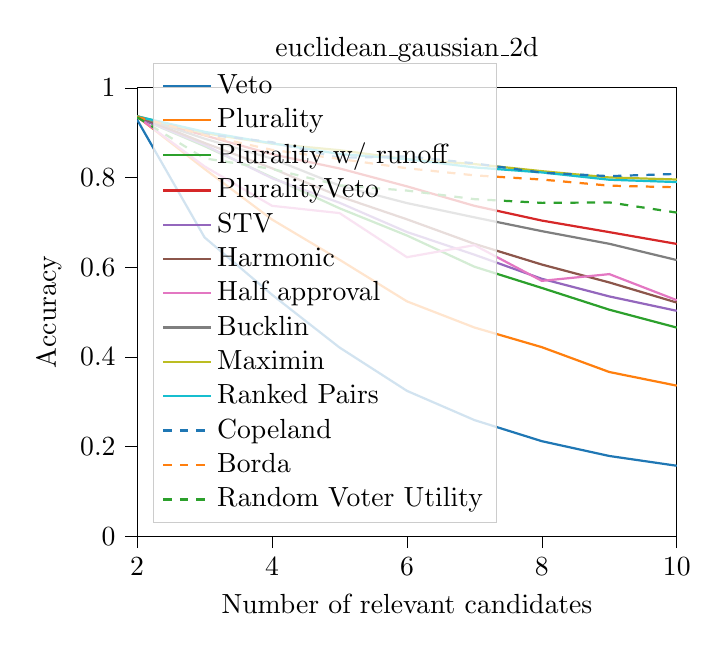
\begin{tikzpicture}

\definecolor{color0}{rgb}{0.12156862745098,0.466666666666667,0.705882352941177}
\definecolor{color1}{rgb}{1,0.498039215686275,0.0549019607843137}
\definecolor{color2}{rgb}{0.172549019607843,0.627450980392157,0.172549019607843}
\definecolor{color3}{rgb}{0.83921568627451,0.152941176470588,0.156862745098039}
\definecolor{color4}{rgb}{0.580392156862745,0.403921568627451,0.741176470588235}
\definecolor{color5}{rgb}{0.549019607843137,0.337254901960784,0.294117647058824}
\definecolor{color6}{rgb}{0.890196078431372,0.466666666666667,0.76078431372549}
\definecolor{color7}{rgb}{0.737254901960784,0.741176470588235,0.133333333333333}
\definecolor{color8}{rgb}{0.0901960784313725,0.745098039215686,0.811764705882353}

\begin{axis}[
legend cell align={left},
legend style={
  fill opacity=0.8,
  draw opacity=1,
  text opacity=1,
  at={(0.03,0.03)},
  anchor=south west,
  draw=white!80!black
},
tick align=outside,
tick pos=left,
title={euclidean\_gaussian\_2d},
x grid style={white!69.0196078431373!black},
xlabel={Number of relevant candidates},
xmin=2, xmax=10,
xtick style={color=black},
y grid style={white!69.0196078431373!black},
ylabel={Accuracy},
ymin=0, ymax=1,
ytick style={color=black}
]
\addplot [thick, color0]
table {%
2 0.929
3 0.6664
4 0.5386
5 0.4209
6 0.3242
7 0.259
8 0.2119
9 0.1789
10 0.1571
};
\addlegendentry{Veto}
\addplot [thick, color1]
table {%
2 0.9363
3 0.8191
4 0.7063
5 0.6167
6 0.5238
7 0.4655
8 0.4216
9 0.3662
10 0.3358
};
\addlegendentry{Plurality}
\addplot [thick, color2]
table {%
2 0.9345
3 0.8701
4 0.8004
5 0.7314
6 0.6707
7 0.6011
8 0.5537
9 0.5052
10 0.4653
};
\addlegendentry{Plurality w/ runoff}
\addplot [thick, color3]
table {%
2 0.9354
3 0.894
4 0.8519
5 0.8203
6 0.7803
7 0.7369
8 0.704
9 0.6782
10 0.6519
};
\addlegendentry{PluralityVeto}
\addplot [thick, color4]
table {%
2 0.9343
3 0.8729
4 0.7984
5 0.7438
6 0.6785
7 0.6279
8 0.5741
9 0.5348
10 0.5027
};
\addlegendentry{STV}
\addplot [thick, color5]
table {%
2 0.9367
3 0.8771
4 0.8206
5 0.758
6 0.7068
7 0.6521
8 0.6059
9 0.566
10 0.5211
};
\addlegendentry{Harmonic}
\addplot [thick, color6]
table {%
2 0.9359
3 0.8248
4 0.7369
5 0.7207
6 0.6223
7 0.6492
8 0.5695
9 0.5846
10 0.5264
};
\addlegendentry{Half approval}
\addplot [thick, white!49.8039215686275!black]
table {%
2 0.9369
3 0.8867
4 0.8422
5 0.7821
6 0.743
7 0.7112
8 0.6804
9 0.6522
10 0.6159
};
\addlegendentry{Bucklin}
\addplot [thick, color7]
table {%
2 0.9366
3 0.8989
4 0.8754
5 0.861
6 0.8407
7 0.83
8 0.8142
9 0.8002
10 0.7956
};
\addlegendentry{Maximin}
\addplot [thick, color8]
table {%
2 0.9364
3 0.902
4 0.8763
5 0.8525
6 0.841
7 0.8226
8 0.8114
9 0.7951
10 0.7899
};
\addlegendentry{Ranked Pairs}
\addplot [thick, color0, dashed]
table {%
2 0.9348
3 0.8969
4 0.8788
5 0.8439
6 0.8472
7 0.8316
8 0.8108
9 0.8031
10 0.8081
};
\addlegendentry{Copeland}
\addplot [thick, color1, dashed]
table {%
2 0.9352
3 0.8949
4 0.8617
5 0.8415
6 0.8207
7 0.8049
8 0.7955
9 0.7819
10 0.7782
};
\addlegendentry{Borda}
\addplot [thick, color2, dashed]
table {%
2 0.9345
3 0.8428
4 0.8191
5 0.7826
6 0.7709
7 0.7518
8 0.7435
9 0.7445
10 0.7218
};
\addlegendentry{Random Voter Utility}
\end{axis}

\end{tikzpicture}
